\documentclass{beamer}


\usepackage{graphicx}
\usepackage{amsmath}
\usepackage{amsfonts}
\usepackage{lmodern}

\usetheme{Rochester}

\usepackage[absolute,overlay]{textpos}
\newenvironment{reference}[2]{%
  \begin{textblock*}{\textwidth}(#1,#2)
    \footnotesize\it\bgroup\color{blue!50!black}}{\egroup\end{textblock*}}

\setbeamertemplate{navigation symbols}{}

\title{CPFSK Softwareradio}
\author{Luckas Becker, Tobias Frahm}
\institute[HAW]{Dept. Informations- und Elektrotechnik\\HAW Hamburg}
\date{\today}


%\frame{
%  \frametitle{FIR-Polyphasen Bandpass}
%  \begin{columns}
%    \begin{column}{0.5\textwidth}
%
%    \end{column}
%    \begin{column}{0.5\textwidth}
%
%    \end{column}
%  \end{columns}
%}

\begin{document}

\frame[plain]{\titlepage}

\section[Outline]{}

\frame{\tableofcontents}

\section{Softwareradio}

\frame{
  \frametitle{Softwareradio}
  \begin{itemize}
  \item<1-> Was ist der Unterschied zu einem normalen Empfänger?
  \end{itemize}
}

\section{Signalfluss Empfänger}
\frame{
  \frametitle{Signalfluss Empfänger}
  \begin{columns}
    \begin{column}{0.3\textwidth}
       \begin{itemize}
         \item 1. FIR-Polyphasen Bandpass
         \item 2. komplexes Kammfilter
         \item 3. FM-Verzögerungsdemodulator
         \item 4. Decodierer
       \end{itemize}
    \end{column}
    \begin{column}{0.7\textwidth}
        \begin{center}
         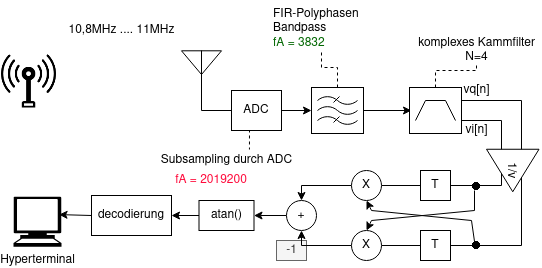
\includegraphics[width=0.6\textwidth]{images/signalfluss.png}
         \end{center}
    \end{column}
  \end{columns}
}
\section{FIR-Polyphasen Bandpass}
\frame{
  \frametitle{FIR-Polyphasen Bandpass}
  \begin{columns}
    \begin{column}{0.5\textwidth}
      \begin{itemize}
        \item in MATLAB Bandpass als FIR-Filter ausgelegt
        \item Dezimationsfaktor bestimmt
        \item Mit Pyhton einen C-Headerfile mit den Polyphasen erzeugt.
      \end{itemize}
    \end{column}
    \begin{column}{0.5\textwidth}
        \begin{itemize}
          \item performanter ANSI-C Code durch Pointerarithmetik
          \item und vermeidung von Schleifen
        \end{itemize}
    \end{column}
  \end{columns}
}

\subsection{FIR Bandpass in MATLAB}
\frame{
  \frametitle{FIR Bandpass in MATLAB}
  \begin{columns}
    \begin{column}{0.5\textwidth}
      Iteratives Vorgehen bis die Koeffizientenanzahl 
      annehmbar war.
      \begin{itemize}
        \item Festlegung der Grenzfrequenzen $f_u = 3800Hz$ und $f_o = 4500Hz$
        \item Abschätzen der Start-/Stopfrequenzen $f_{start/stop} = f_{u/o} \pm 1500Hz$.
      \end{itemize}
    \end{column}
    \begin{column}{0.5\textwidth}
      Bei dem hier gezeigten Amplitudengang werden 2056 Koeffizienten benötigt.
      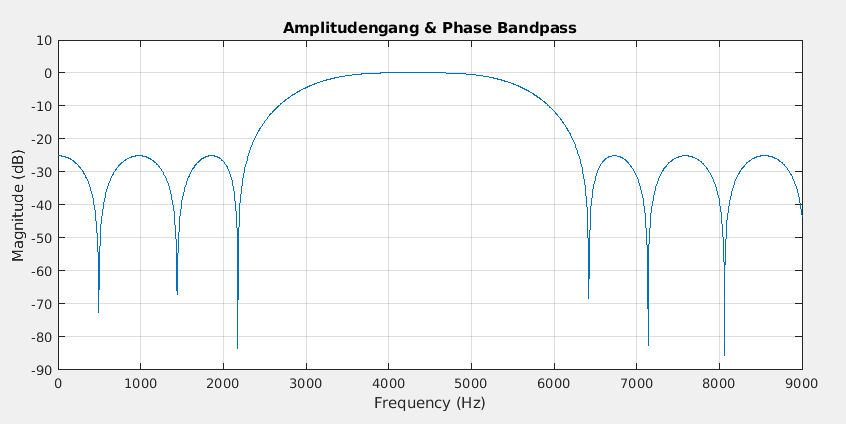
\includegraphics[width=\textwidth]{images/FIR_BP.png}
    \end{column}
  \end{columns}
}

\subsection{FIR-Polyphasen Bandpass in ANSI-C}
\frame{
  \frametitle{FIR-Polyphasen Bandpass in ANSI-C}
  \begin{columns}
    \begin{column}{0.5\textwidth}
      Zunächst werden die Koeffizienten des FIR-Bandpass exportiert.
      Anschließend mithilfe eines Pythonscripts in $527$ Polyphasen
      aufgeteilt, ggf. mit nullen aufgefüllt, und als \textit{const char}-Arrays
      in ein C-File exportiert.
    \end{column}
    \begin{column}{0.5\textwidth}
      \begin{itemize}
        \item \textit{const char} für effiziente Speichernutzung
        \item effizienter Zugriff nur durch Pointerreferenz
      \end{itemize}
    \end{column}
  \end{columns}
}


\section{Hilbert Transformator}
\section{Komplexes Kammfilter}
\section{FM-Verzögerungsdemodulator}
\section{Decodierer}

\nocite{*} % Include everything in the .bib file.

\bibliographystyle{plainnat}
\bibliography{presentation}

% that's all, folks
\end{document}
